\documentclass[11pt,a4paper]{article}

% --- Packages ---
\usepackage[utf8]{inputenc}
\usepackage[T1]{fontenc}
\usepackage{amsmath,amssymb,amsthm}
\usepackage{mathtools}
\usepackage{geometry}
\usepackage{hyperref}
\usepackage{booktabs}
\usepackage{enumitem}
\usepackage{algorithm}
\usepackage{algpseudocode}
\usepackage{xcolor}
\usepackage{tcolorbox}
\usepackage{fancyhdr}
\usepackage{titlesec}
\usepackage{tikz}
\usetikzlibrary{arrows.meta,positioning,calc,fit,backgrounds,decorations.pathreplacing,shapes.geometric}

\geometry{margin=2.5cm}
\hypersetup{colorlinks=true, linkcolor=blue!70!black, citecolor=green!50!black, urlcolor=blue!60!black}

% --- Theorem environments ---
\theoremstyle{definition}
\newtheorem{definition}{Definition}[section]
\newtheorem{remark}{Remark}[section]

% --- Custom commands ---
\newcommand{\E}{\mathbb{E}}
\newcommand{\Var}{\mathrm{Var}}
\newcommand{\KL}{\mathrm{KL}}
\newcommand{\R}{\mathbb{R}}
\newcommand{\bx}{\mathbf{x}}
\newcommand{\by}{\mathbf{y}}
\newcommand{\bw}{\mathbf{w}}
\newcommand{\bX}{\mathbf{X}}
\newcommand{\bK}{\mathbf{K}}
\newcommand{\bI}{\mathbf{I}}
\newcommand{\bmu}{\boldsymbol{\mu}}
\newcommand{\bsigma}{\boldsymbol{\sigma}}
\newcommand{\btheta}{\boldsymbol{\theta}}
\newcommand{\bphi}{\boldsymbol{\phi}}
\newcommand{\bpi}{\boldsymbol{\pi}}
\newcommand{\softmax}{\mathrm{softmax}}
\newcommand{\sigmoid}{\mathrm{sigmoid}}
\newcommand{\diag}{\mathrm{diag}}
\DeclareMathOperator*{\argmax}{arg\,max}
\DeclareMathOperator*{\argmin}{arg\,min}
\DeclareMathOperator{\sign}{sign}
\DeclareMathOperator{\erfc}{erfc}
\DeclareMathOperator{\softplus}{softplus}

% --- Code reference style ---
\newtcolorbox{implnote}{colback=gray!5, colframe=gray!50, title=Implementation Note, fonttitle=\bfseries\small}

% --- Diagram color palette ---
\definecolor{inputcol}{HTML}{4A90D9}
\definecolor{classcol}{HTML}{E67E22}
\definecolor{regcol}{HTML}{27AE60}
\definecolor{aggcol}{HTML}{8E44AD}
\definecolor{gatecol}{HTML}{C0392B}
\definecolor{losscol}{HTML}{2C3E50}
\definecolor{treecol}{HTML}{16A085}
\definecolor{flexcol}{HTML}{2980B9}

\tikzset{
  block/.style={
    rectangle, draw=#1, fill=#1!10, thick,
    minimum height=0.9cm, minimum width=2.2cm,
    text centered, font=\small\sffamily,
    rounded corners=3pt,
  },
  smallblock/.style={
    rectangle, draw=#1, fill=#1!10, thick,
    minimum height=0.65cm, minimum width=1.4cm,
    text centered, font=\footnotesize\sffamily,
    rounded corners=2pt,
  },
  arr/.style={-{Stealth[length=2.5mm]}, thick, #1},
  arr/.default={black},
  darr/.style={-{Stealth[length=2mm]}, thick, densely dashed, #1},
  darr/.default={gray},
  tensor/.style={font=\tiny\ttfamily, text=gray!70!black},
}

% --- Header ---
\pagestyle{fancy}
\fancyhf{}
\fancyhead[L]{\small Mathematical Guide --- AutoML Package}
\fancyhead[R]{\small\thepage}
\renewcommand{\headrulewidth}{0.4pt}

% --- Part styling ---
\titleclass{\part}{top}
\titleformat{\part}[display]{\centering\Large\bfseries}{Part \thepart}{10pt}{\LARGE}
\titlespacing*{\part}{0pt}{20pt}{20pt}

% --- Title ---
\title{\textbf{Mathematical Guide} \\ \Large All Models, Losses, Strategies, and Uncertainty Methods \\ \large in the AutoML Package}
\author{AutoML Research Project}
\date{April 2026}

\begin{document}
\maketitle
\tableofcontents
\newpage

%#############################################################################
\part{Framework}
%#############################################################################

%=============================================================================
\section{Introduction and Notation}
%=============================================================================

This document provides a complete mathematical specification of every model,
loss function, selection strategy, uncertainty method, and evaluation metric
in the AutoML package --- both currently implemented and proposed.

\subsection{Notation}

\begin{center}
\begin{tabular}{cl}
\toprule
Symbol & Meaning \\
\midrule
$\bx \in \R^d$ & Input feature vector ($d$ features) \\
$y \in \R$ & Scalar regression target \\
$N$ & Number of training samples \\
$K$ & Number of classes / bins / mixture components \\
$D$ & Number of hidden layers (depth) in FlexibleNN \\
$M$ & Number of ensemble members or MC samples \\
$\pi_k(\bx)$ & Probability of class $k$ given input $\bx$ \\
$\mu_k(\bx)$ & Mean prediction of regression head $k$ \\
$\sigma_k^2(\bx)$ & Variance prediction of regression head $k$ \\
$\hat{y}(\bx)$ & Final point prediction \\
$\hat{\sigma}^2(\bx)$ & Final variance prediction \\
$\btheta$ & All learnable parameters \\
$\bphi$ & Parameters of a selection / gating subnetwork \\
$\tau$ & Temperature parameter (Gumbel-Softmax) \\
$\alpha$ & Miscoverage level for prediction intervals \\
$\beta$ & Variance weighting exponent ($\beta$-NLL) \\
$k(\bx, \bx')$ & Kernel / covariance function (GP) \\
$\eta$ & Learning rate \\
\bottomrule
\end{tabular}
\end{center}

Tensor shapes are written in parentheses: $(B, K)$ means batch size $B$, $K$
columns. We write $[n]$ for $\{1, 2, \ldots, n\}$.

%=============================================================================
\section{Uncertainty Quantification: A Unified View}
\label{sec:uq}
%=============================================================================

Every model in this package produces (or can produce) an uncertainty estimate
$\hat{\sigma}^2(\bx)$. This section provides the taxonomy \emph{before}
describing individual models, so the reader has the mental model up front.

\subsection{Taxonomy of Uncertainty Sources}

\begin{center}
\renewcommand{\arraystretch}{1.3}
\begin{tabular}{lp{4.2cm}p{4.2cm}c}
\toprule
\textbf{Method} & \textbf{How $\hat{\sigma}^2$ is produced} & \textbf{What it captures} & \textbf{Input-dep?} \\
\midrule
Learned variance (NLL) & Second output of NN, trained via NLL & Aleatoric & Yes \\
Law of Total Variance & Aggregation of per-class $(\mu_k, \sigma_k^2)$ & Aleatoric + epistemic-like & Yes \\
MC Dropout & Empirical variance of $M$ stochastic passes & Epistemic (approx.) & Yes \\
Deep Ensembles & Variance across $M$ independent models & Aleatoric + epistemic & Yes \\
Binned Residual Std & Variance of training residuals in bins & Aleatoric (discretized) & Partially \\
Lookup Mapper & Per-probability-bin variance & Aleatoric (discretized) & Partially \\
GP Posterior & Analytical posterior variance & Aleatoric + epistemic & Yes \\
Conformal & Calibration-set residual quantile & Coverage guarantee & No (marginal) \\
Constant & Global scalar, not learned & None (placeholder) & No \\
\bottomrule
\end{tabular}
\end{center}

\subsection{Learned Variance via NLL}
\label{sec:uq_nll}

The network outputs $(\mu(\bx), \log\sigma^2(\bx))$ and is trained with
the Gaussian NLL (\S\ref{sec:nll}). The gradient w.r.t.\ $\log\sigma^2$:
\[
  \frac{\partial \mathcal{L}}{\partial \log\sigma^2} = \frac{1}{2}\left(1 - \frac{(y - \mu)^2}{\sigma^2}\right),
\]
drives $\sigma^2$ toward $\E[(y - \mu)^2 \mid \bx]$, the true conditional
variance, at convergence.

\textbf{Used by:} ProbReg (per-head), Plain NN (\texttt{PROBABILISTIC}),
NN Mapper, Deep Ensembles (per member), NGBoost, tree models (custom objective).

\subsection{Law of Total Variance}
\label{sec:uq_lotv}

Given per-class predictions $\{(\mu_k, \sigma_k^2)\}_{k=1}^{K}$ weighted by
$\{\pi_k\}_{k=1}^{K}$:
\begin{align}
  \hat{\sigma}^2 &= \underbrace{\sum_k \pi_k \sigma_k^2}_{\text{expected within-class variance}} + \underbrace{\sum_k \pi_k (\mu_k - \hat{y})^2}_{\text{between-class variance}}.
\end{align}

The first term is aleatoric (noise within each class). The second term
captures disagreement among class means. When all $\mu_k$ agree, the
second term vanishes and we get pure aleatoric uncertainty.

\textbf{Used by:} ProbReg (central novelty), MDN, Deep Ensembles (with
uniform $\pi_m = 1/M$).

\subsection{MC Dropout}
\label{sec:uq_mcdropout}

Gal \& Ghahramani (2016): keep dropout active at test time and run $M$
forward passes:
\begin{align}
  \hat{y}_m &= f_{\btheta, \mathbf{z}_m}(\bx), \quad \mathbf{z}_m \sim \text{Bernoulli}(1-p)^L, \quad m = 1, \ldots, M, \\
  \hat{\mu} &= \frac{1}{M}\sum_{m=1}^M \hat{y}_m, \qquad
  \hat{\sigma}^2 = \frac{1}{M}\sum_{m=1}^M (\hat{y}_m - \hat{\mu})^2.
\end{align}

\textbf{Used by:} Plain NN (with \texttt{MC\_DROPOUT}).

\subsection{Binned Residual Standard Deviation}
\label{sec:uq_binned}

A post-hoc method. After training:
\begin{enumerate}[nosep]
  \item Compute residuals: $r_i = y_i - \hat{y}_i$ for all training samples.
  \item Bin predictions into $B$ bins by $\hat{y}_i$.
  \item For each bin $b$: $\hat{\sigma}_b = \mathrm{std}(\{r_i : \hat{y}_i \in b\})$.
  \item At test time: $\hat{\sigma}(\bx) = \hat{\sigma}_{b(\hat{y}(\bx))}$.
\end{enumerate}

\textbf{Partially input-dependent:} piecewise constant (one value per bin).

\textbf{Used by:} Linear Regression, XGBoost, LightGBM, CatBoost, Plain NN
(with \texttt{BINNED\_RESIDUAL\_STD}).

\subsection{Summary: How Each Model Produces Uncertainty}

\begin{center}
\renewcommand{\arraystretch}{1.3}
\footnotesize
\begin{tabular}{lll}
\toprule
\textbf{Model} & \textbf{Primary UQ Method} & \textbf{Alternatives} \\
\midrule
Linear Regression & Binned Residual Std & --- \\
Plain NN & Depends on \texttt{uncertainty\_method} & CONSTANT / PROBABILISTIC / MC\_DROPOUT / BINNED \\
XGBoost & Custom NLL objective (learned $\sigma^2$) & Binned Residual Std \\
LightGBM & Custom NLL objective (learned $\sigma^2$) & Binned Residual Std \\
CatBoost & Custom NLL objective (learned $\sigma^2$) & Binned Residual Std \\
ProbReg & Law of Total Variance & + Conformal wrapper \\
ClassReg (Lookup) & Per-bin variance from lookup table & Conformal wrapper \\
ClassReg (Spline) & Constant residual variance & --- \\
ClassReg (NN Mapper) & Learned $\sigma^2$ via NLL & --- \\
FlexibleNN & Same as Plain NN & --- \\
GP & Posterior variance (analytical) & --- \\
Deep Ensembles & Ensemble disagreement + mean aleatoric & --- \\
NGBoost & Natural gradient learned $\sigma^2$ & --- \\
MDN & Mixture variance (law of total variance) & --- \\
Quantile Regression & Quantile-based intervals & --- \\
\bottomrule
\end{tabular}
\end{center}

%#############################################################################
\part{Currently Supported Models}
%#############################################################################

%=============================================================================
\section{Linear Regression}
%=============================================================================

Ordinary least squares:
\[
  \hat{y} = \bw^\top \bx + b, \quad (\bw, b) = \argmin_{\bw, b} \sum_{i=1}^{N} (y_i - \bw^\top \bx_i - b)^2.
\]

\textbf{Uncertainty:} No native uncertainty. Uses post-hoc
\texttt{BINNED\_RESIDUAL\_STD} (\S\ref{sec:uq_binned}).

%=============================================================================
\section{Gradient-Boosted Trees (XGBoost, LightGBM, CatBoost)}
\label{sec:gbt}
%=============================================================================

All three share the same additive ensemble structure:
\[
  \hat{y}(\bx) = \sum_{t=1}^{T} \eta \cdot f_t(\bx), \quad f_t \in \mathcal{F},
\]
where $\mathcal{F}$ is the space of decision trees, $\eta$ is the learning rate
(shrinkage), and each tree $f_t$ is fit to the pseudo-residuals.

\subsection{Regularized Objective}

At step $t$:
\begin{equation}
  \mathcal{L}^{(t)} = \sum_{i=1}^{N} \left[g_i f_t(\bx_i) + \frac{1}{2} h_i f_t(\bx_i)^2\right] + \gamma T_{\mathrm{leaves}} + \frac{1}{2}\lambda \sum_{j=1}^{T_{\mathrm{leaves}}} w_j^2,
  \label{eq:xgb_obj}
\end{equation}
where $g_i = \partial \mathcal{L} / \partial \hat{y}_i$ and $h_i = \partial^2 \mathcal{L} / \partial \hat{y}_i^2$.

\subsection{Custom NLL Objective for Probabilistic Output}
\label{sec:tree_nll}

For trees predicting $(\mu, \log\sigma^2)$, custom gradients and Hessians:

\textbf{Mean output:}
\begin{align}
  g_\mu &= \frac{\mu - y}{\sigma^2}, &
  h_\mu &= \frac{1}{\sigma^2}.
\end{align}

\textbf{Log-variance output:}
\begin{align}
  g_{\log\sigma^2} &= \frac{1}{2}\left(1 - \frac{(y - \mu)^2}{\sigma^2}\right), &
  h_{\log\sigma^2} &= \frac{1}{2} \quad \text{(Fisher information)}.
  \label{eq:tree_hessian}
\end{align}

\begin{implnote}
Bug N5: the current implementation uses the observed Hessian
$h = \frac{1}{2}\frac{(y-\mu)^2}{\sigma^2}$ instead of the Fisher
information $h = \frac{1}{2}$. The Fisher information is preferred because
it is always positive and gives more stable tree splits.
\end{implnote}

\subsection{Implementation Differences}

\begin{itemize}[nosep]
  \item \textbf{XGBoost} (Chen \& Guestrin, 2016): exact or approximate greedy split finding, L1/L2 regularization on leaf weights.
  \item \textbf{LightGBM} (Ke et al., 2017): histogram-based splits, gradient-based one-side sampling (GOSS), exclusive feature bundling (EFB).
  \item \textbf{CatBoost} (Prokhorenkova et al., 2018): ordered boosting to prevent target leakage, oblivious (symmetric) trees with balanced splits at each depth.
\end{itemize}

\textbf{Uncertainty:} Learned $\sigma^2(\bx)$ via custom NLL objective, or
post-hoc \texttt{BINNED\_RESIDUAL\_STD}.

%=============================================================================
\section{Plain PyTorch Neural Network}
%=============================================================================

A feedforward MLP:
\[
  f_\btheta(\bx) = W_L \cdot \sigma(W_{L-1} \cdots \sigma(W_1 \bx + b_1) \cdots + b_{L-1}) + b_L,
\]
where $\sigma$ is an activation function (ReLU, GELU, etc.) and $L$ is the
number of layers.

\textbf{Uncertainty modes:}
\begin{itemize}[nosep]
  \item \texttt{CONSTANT}: No learned uncertainty. $\hat{\sigma}^2$ is a global constant.
  \item \texttt{PROBABILISTIC}: Output layer produces $(\mu, \log\sigma^2)$; trained with Gaussian NLL (\S\ref{sec:uq_nll}).
  \item \texttt{MC\_DROPOUT}: Dropout active at test time; run $M$ forward passes (\S\ref{sec:uq_mcdropout}).
  \item \texttt{BINNED\_RESIDUAL\_STD}: Post-hoc binned variance (\S\ref{sec:uq_binned}).
\end{itemize}

%=============================================================================
\section{Classifier-Regression Model}
\label{sec:classreg}
%=============================================================================

A two-stage model: (1) discretize the target into bins and train a
classifier, (2) map classifier probabilities back to regression predictions.

\subsection{Architecture Overview}

\begin{figure}[ht]
\centering
\resizebox{0.92\textwidth}{!}{%
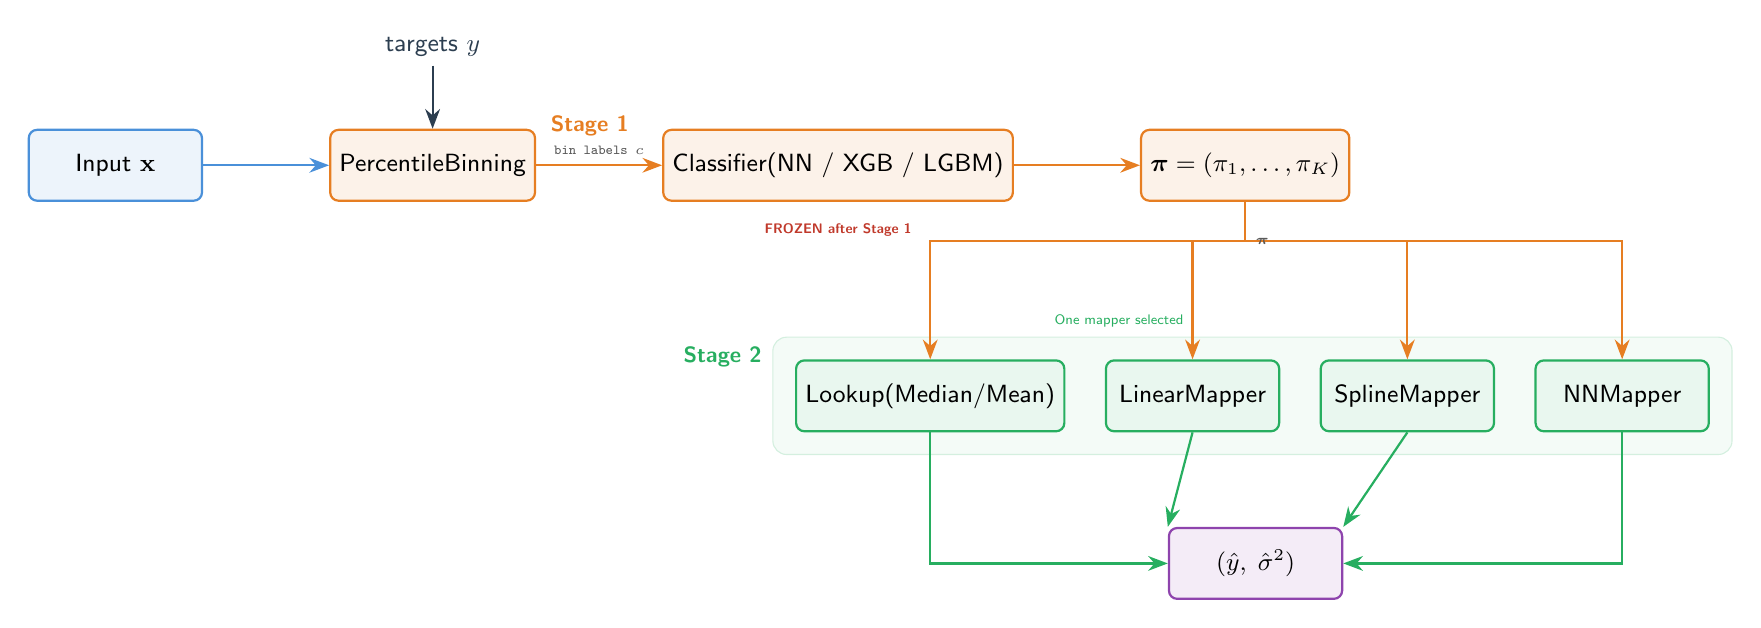
\begin{tikzpicture}[node distance=0.9cm and 1.4cm]

% ===== Stage 1 =====
\node[block=inputcol] (input) {Input $\bx$};
\node[block=classcol, right=1.6cm of input] (binning) {Percentile\\Binning};
\node[block=classcol, right=1.6cm of binning] (clf) {Classifier\\(NN / XGB / LGBM)};
\node[block=classcol, right=1.6cm of clf] (probs) {$\bpi = (\pi_1, \ldots, \pi_K)$};

\node[above=0.8cm of binning, font=\small\sffamily, text=losscol] (target) {targets $y$};
\draw[arr=losscol] (target) -- (binning);

\draw[arr=inputcol] (input) -- (binning);
\draw[arr=classcol] (binning) -- (clf) node[midway, above, tensor] {bin labels $c$};
\draw[arr=classcol] (clf) -- (probs);

\node[below=0.15cm of clf, font=\tiny\sffamily\bfseries, text=gatecol] {FROZEN after Stage 1};

% ===== Stage 2: Mappers =====
\node[block=regcol, below=2.0cm of probs, xshift=-4cm] (lookup) {Lookup\\(Median/Mean)};
\node[block=regcol, right=0.5cm of lookup] (linear) {Linear\\Mapper};
\node[block=regcol, right=0.5cm of linear] (spline) {Spline\\Mapper};
\node[block=regcol, right=0.5cm of spline] (nnmap) {NN\\Mapper};

\draw[arr=classcol] (probs.south) -- ++(0,-0.5) -| (lookup.north);
\draw[arr=classcol] (probs.south) -- ++(0,-0.5) -| (linear.north);
\draw[arr=classcol] (probs.south) -- ++(0,-0.5) -| (spline.north);
\draw[arr=classcol] (probs.south) -- ++(0,-0.5) -| (nnmap.north)
  node[pos=0.0, right, tensor] {$\bpi$};

% ===== Output =====
\node[block=aggcol, below=1.2cm of linear, xshift=0.8cm] (out) {$(\hat{y},\; \hat{\sigma}^2)$};
\draw[arr=regcol] (lookup.south) |- (out.west);
\draw[arr=regcol] (linear.south) -- (out.north west);
\draw[arr=regcol] (spline.south) -- (out.north east);
\draw[arr=regcol] (nnmap.south) |- (out.east);

\node[left=0.3cm of clf, yshift=0.5cm, font=\footnotesize\sffamily\bfseries, text=classcol] {Stage 1};
\node[left=0.3cm of lookup, yshift=0.5cm, font=\footnotesize\sffamily\bfseries, text=regcol] {Stage 2};

\begin{scope}[on background layer]
  \node[fit=(lookup)(nnmap), fill=regcol!5, draw=regcol!20,
    rounded corners=5pt, inner sep=8pt,
    label={[font=\tiny\sffamily,text=regcol]above left:One mapper selected}] {};
\end{scope}

\end{tikzpicture}
}%
\caption{ClassifierRegression two-stage architecture. The classifier is frozen before Stage 2 (mapper) training.}
\label{fig:classreg}
\end{figure}

\subsection{Binning}

Targets are binned using percentile-based boundaries:
\begin{align}
  q_j &= \text{Percentile}\left(y_{\mathrm{train}}, \frac{100 \cdot j}{K}\right), \quad j = 0, 1, \ldots, K, \\
  c_i &= \max\{j : y_i \geq q_j\}, \quad c_i \in \{0, 1, \ldots, K-1\}.
\end{align}

Duplicate boundaries (from repeated values) are collapsed, and $K$ is
reduced accordingly.

\subsection{Stage 1: Classification}

Train a classifier $f: \R^d \to \Delta^K$ (NN, XGBoost, LightGBM, or
CatBoost) on $(\bx_i, c_i)$ pairs. After training, \textbf{freeze} the classifier.

\subsection{Stage 2: Mapping}

A \emph{mapper} transforms class probabilities to regression predictions.

\subsubsection{Linear Mapper}

$\hat{y} = a \cdot \hat{\pi} + b$, where $\hat{\pi}$ is a scalar summary
of the probability vector and $(a, b)$ are fit by OLS.

\textbf{Uncertainty:} Constant residual variance $\hat{\sigma}^2 = \frac{1}{N}\sum_i(y_i - \hat{y}_i)^2$.

\subsubsection{Lookup Mapper (\texttt{LOOKUP\_MEDIAN} / \texttt{LOOKUP\_MEAN})}

The most reliable mapper. Bins the probability space and computes per-bin statistics:

\begin{enumerate}[nosep]
  \item For each class $k$, collect $\pi_k(\bx_i)$ across training samples.
  \item Bin the probability values into $B$ bins (where $B = \max(B_{\min}, \min(B_{\max}, N/100))$).
  \item For each bin $b$:
    \begin{align}
      \hat{y}_b &= \mathrm{median}(\{y_i : \pi_k(\bx_i) \in b\}) \quad \text{(or mean)}, \\
      \hat{\sigma}^2_b &= \mathrm{var}(\{y_i : \pi_k(\bx_i) \in b\}) \quad \text{(if PROBABILISTIC)}.
    \end{align}
  \item At prediction time: look up the bin for $\pi_k(\bx)$, return $(\hat{y}_b, \hat{\sigma}^2_b)$.
\end{enumerate}

\textbf{Uncertainty:} Per-probability-bin variance --- \emph{input-dependent}
through the probability: different $\pi_k$ values land in different bins.

\subsubsection{Spline Mapper}

$\hat{y} = S(\pi_k; \text{degree}=k_s, \text{smoothing}=s)$ via
\texttt{UnivariateSpline}. Known to be unstable.

\textbf{Uncertainty:} Constant residual variance (no per-input variance).

\subsubsection{Neural Network Mapper}

$(\hat{y}, \log\hat{\sigma}^2) = h_\btheta(\bpi)$ where $h$ is a small MLP.
Trained with NLL loss (probabilistic) or MSE (deterministic).

\textbf{Uncertainty:} Learned input-dependent $\hat{\sigma}^2$ via NLL.
Known training issues due to two-stage optimization.

%=============================================================================
\section{Probabilistic Regression Model (ProbReg)}
\label{sec:probreg}
%=============================================================================

The central idea: discretize the prediction task into $K$ classes via a
learned classifier, attach a per-class regression head that outputs
$(\mu_k, \log\sigma_k^2)$, and combine via the \textbf{law of total variance}.

\subsection{Architecture Overview}

\begin{figure}[ht]
\centering
\resizebox{\textwidth}{!}{%
\begin{tikzpicture}[node distance=1.0cm and 1.6cm]

\node[block=inputcol] (input) {Input $\bx \in \R^d$};
\node[block=classcol, right=1.8cm of input] (classifier) {Classifier NN\\$f_\btheta(\bx)$};
\draw[arr=inputcol] (input) -- (classifier) node[midway, above, tensor] {$(B, d)$};

\node[block=classcol, right=1.8cm of classifier] (softmax) {Masked Softmax\\$\pi_k = \softmax(\tilde{\ell})_k$};
\draw[arr=classcol] (classifier) -- (softmax) node[midway, above, tensor] {$(B, K)$ logits};

\node[block=gatecol, above=1.3cm of classifier] (gate) {$K$-Predictor $g_\bphi(\bx)$};
\draw[arr=inputcol] (input.north) |- (gate.west);
\draw[darr=gatecol] (gate.east) -| (softmax.north)
  node[pos=0.75, right, font=\footnotesize\sffamily, text=gatecol] {mask $k > K^*$};
\node[above=0.1cm of gate, font=\tiny\sffamily, text=gatecol, align=center]
  {SoftGating / Gumbel / STE / REINFORCE};

\node[smallblock=gatecol, right=1.2cm of gate] (kl) {$\KL(q \| p)$};
\draw[darr=gatecol] (gate) -- (kl);

\node[block=regcol, below=1.8cm of softmax, xshift=-1.4cm] (head1) {$h_1$: $(\mu_1, \log\sigma_1^2)$};
\node[block=regcol, right=0.3cm of head1] (head2) {$h_2$: $(\mu_2, \log\sigma_2^2)$};
\node[right=0.3cm of head2, font=\large] (dots) {$\cdots$};
\node[block=regcol, right=0.3cm of dots] (headk) {$h_K$: $(\mu_K, \log\sigma_K^2)$};

\draw[arr=classcol] (softmax.south) -- ++(0,-0.5) -| (head1.north)
  node[near start, left, tensor] {$\pi_1$};
\draw[arr=classcol] (softmax.south) -- ++(0,-0.5) -| (head2.north);
\draw[arr=classcol] (softmax.south) -- ++(0,-0.5) -| (headk.north)
  node[near start, right, tensor] {$\pi_K$};

\node[block=aggcol, below=1.8cm of head2, xshift=0.5cm, minimum width=5cm] (lotv)
  {\begin{tabular}{c}\textbf{Law of Total Variance}\\[2pt]
  $\hat{y} = \sum_k \pi_k \mu_k$ \quad
  $\hat{\sigma}^2 = \sum_k \pi_k \sigma_k^2 + \sum_k \pi_k(\mu_k - \hat{y})^2$
  \end{tabular}};

\draw[arr=regcol] (head1.south) |- ([yshift=0.25cm]lotv.west) -- (lotv.west);
\draw[arr=regcol] (head2.south) -- (lotv.north);
\draw[arr=regcol] (headk.south) |- ([yshift=0.25cm]lotv.east) -- (lotv.east);

\draw[darr=classcol] (softmax.east) -- ++(0.5,0) -- ++(0,-4.2) -| (lotv.south east)
  node[pos=0.45, right, tensor] {$\bpi$};

\node[block=aggcol, below=1.0cm of lotv] (output) {$(\hat{y},\; \hat{\sigma}^2)$};
\draw[arr=aggcol] (lotv) -- (output) node[midway, right, tensor] {$(B, 2)$};

\node[block=losscol, left=1.8cm of output] (loss)
  {$\mathcal{L} = \mathcal{L}_{\mathrm{NLL}} + \lambda_{\mathrm{CE}}\mathcal{L}_{\mathrm{CE}} + \lambda_{\mathrm{KL}}\KL$};
\draw[arr=losscol] (output) -- (loss);
\draw[darr=gatecol] (kl.north) -- ++(0,0.4) -| ([xshift=-2.5cm]kl.north)
  -- ++(0,-0.4) |- (loss.north);

\begin{scope}[on background layer]
  \node[fit=(head1)(headk)(dots), fill=regcol!5, draw=regcol!30,
    rounded corners=5pt, inner sep=6pt] {};
  \node[fit=(gate)(kl), fill=gatecol!5, draw=gatecol!20,
    rounded corners=5pt, inner sep=6pt,
    label={[font=\tiny\sffamily,text=gatecol]below left:Dynamic $K$ (optional)}] {};
\end{scope}

\end{tikzpicture}
}%
\caption{ProbReg architecture. Solid arrows: data flow. Dashed: optional dynamic-$K$ path.
Each regression head $h_k$ receives only its own probability $\pi_k$ (SEPARATE\_HEADS strategy).}
\label{fig:probreg}
\end{figure}

\begin{enumerate}
  \item \textbf{Classifier backbone} $f_\btheta: \R^d \to \R^K$. Produces raw
        logits $\ell_1, \ldots, \ell_K$. Softmax gives class probabilities:
        \[
          \pi_k(\bx) = \frac{\exp(\ell_k(\bx))}{\sum_{j=1}^{K} \exp(\ell_j(\bx))}.
        \]
  \item \textbf{Regression module} (one of three strategies, \S\ref{sec:reg_strategies}).
  \item \textbf{Aggregation} via law of total variance (\S\ref{sec:uq_lotv}).
  \item \textbf{Optional: dynamic $K$} via a gating subnetwork (\S\ref{sec:dynamic_k}).
\end{enumerate}

\subsection{Class Masking for Variable $K$}

When using dynamic $K$ or a fixed $K < K_{\max}$, classes $k > K$ are masked:
\[
  \tilde{\ell}_k =
  \begin{cases}
    \ell_k & \text{if } k \leq K, \\
    -\infty & \text{if } k > K.
  \end{cases}
\]

\subsection{Regression Strategies}
\label{sec:reg_strategies}

Given class probabilities $\pi_1, \ldots, \pi_K$, the regression module
maps these to per-class outputs $(\mu_k, \log\sigma_k^2)$ for $k \in [K]$.

\subsubsection{Strategy 1: Separate Heads (\texttt{SEPARATE\_HEADS})}

Each class $k$ has an \emph{independent} neural network head $h_k$:
\[
  h_k : \R \to \R^2, \quad h_k(\pi_k) = (\mu_k, \log\sigma_k^2).
\]
The input to head $k$ is the \emph{scalar} probability $\pi_k(\bx)$.
Heads do not share parameters.

\begin{implnote}
This is the primary strategy used in benchmarks. The key architectural choice:
each head only sees its own class probability, not the full probability vector.
The classifier acts as a nonlinear feature extractor projecting onto the
probability simplex; each head learns a scalar-to-scalar function.
\end{implnote}

\subsubsection{Strategy 2: Single Head, $N$ Outputs (\texttt{SINGLE\_HEAD\_N\_OUTPUTS})}

One shared neural network takes the full probability vector:
\[
  h : \R^K \to \R^{K \times 2}, \quad h(\bpi) = \{(\mu_k, \log\sigma_k^2)\}_{k=1}^{K}.
\]

\subsubsection{Strategy 3: Single Head, Final Output (\texttt{SINGLE\_HEAD\_FINAL\_OUTPUT})}

One shared network maps probabilities to per-class representations:
\[
  h : \R^K \to \R^{K \times 2}, \quad
  \hat{y} = \sum_{k=1}^{K} \pi_k \cdot h_k(\bpi).
\]

\begin{remark}
Strategies 2 and 3 allow parameter sharing across classes but lose
the per-class specialization that makes \texttt{SEPARATE\_HEADS} effective.
\end{remark}

\subsection{Law of Total Variance Aggregation}

\begin{definition}[Law of Total Variance Decomposition]
\begin{align}
  \hat{y}(\bx) &= \E[Y \mid \bx] = \sum_{k=1}^{K} \pi_k(\bx) \cdot \mu_k(\bx)
  \label{eq:lotv_mean} \\[6pt]
  \hat{\sigma}^2(\bx) &= \Var(Y \mid \bx) = \underbrace{\sum_{k=1}^{K} \pi_k(\bx) \cdot \sigma_k^2(\bx)}_{\text{expected aleatoric variance}} + \underbrace{\sum_{k=1}^{K} \pi_k(\bx) \cdot (\mu_k(\bx) - \hat{y}(\bx))^2}_{\text{variance of means (epistemic-like)}}
  \label{eq:lotv_var}
\end{align}
\end{definition}

\begin{implnote}
In \texttt{pytorch\_utils.apply\_law\_of\_total\_variance}:
input shapes: probabilities $(B, K)$, per-head outputs $(B, K, 2)$.
Output: $(\hat{y}, \log\hat{\sigma}^2)$ with shape $(B, 2)$, where
$\log\hat{\sigma}^2 = \log(\max(\hat{\sigma}^2, 10^{-9}))$.
\end{implnote}

\subsection{Gradient Stop Variant}

When \texttt{optimization\_strategy = GRADIENT\_STOP}:
$\tilde{\pi}_k = \mathrm{stopgrad}(\pi_k)$.
The classifier is updated only by cross-entropy; regression heads only by NLL.

\subsection{Monotonic Constraints}

Separate mean and variance heads with monotonic linear on the mean:
\begin{align}
  \mu_k &= g_{\mu}(\pi_k; \bw_\mu) \quad \text{(monotonic)}, \qquad
  \log\sigma_k^2 = g_{\sigma}(\pi_k; \bw_\sigma) \quad \text{(unconstrained)}.
\end{align}

Monotonic linear:
\[
  f_{\text{mono}}(\bx; \bw, b) =
  \begin{cases}
    \softplus(\bw)^\top \bx + b & \text{positive monotonicity}, \\
    -\softplus(\bw)^\top \bx + b & \text{negative monotonicity},
  \end{cases}
\]
where $\softplus(w) = \log(1 + e^w)$ ensures non-negative weights.

\subsection{Boundary Constraints}

\texttt{HARDSIGMOID} constrains predictions to $[y_{\min}, y_{\max}]$:
\[
  \tilde{\mu}_k = y_{\min} + (y_{\max} - y_{\min}) \cdot \mathrm{hardsigmoid}(\mu_k).
\]

\textbf{Uncertainty:} Law of total variance (\S\ref{sec:uq_lotv}) ---
the central novelty of ProbReg.

%=============================================================================
\section{Flexible Neural Network (FlexibleNN)}
\label{sec:flexnn}
%=============================================================================

A neural network with \emph{learnable depth}: a gating subnetwork
predicts how many hidden layers each input should use.

\subsection{Architecture}

\begin{figure}[ht]
\centering
\resizebox{0.95\textwidth}{!}{%
\begin{tikzpicture}[node distance=0.9cm and 1.4cm]

\node[block=inputcol] (input) {Input $\bx$};

\node[block=gatecol, above=1.5cm of input, xshift=3cm] (gate) {Gate $g_\bphi(\bx)$};
\draw[arr=inputcol] (input.north) -- ++(0,0.4) -| (gate.south);

\node[smallblock=gatecol, right=1.2cm of gate] (probs) {$\mathbf{p} = \softmax(\ell)$};
\draw[arr=gatecol] (gate) -- (probs);

\node[block=flexcol, right=2.5cm of input] (b1) {Block $B_1$};
\node[block=flexcol, right=0.6cm of b1] (b2) {Block $B_2$};
\node[right=0.4cm of b2, font=\large] (bdots) {$\cdots$};
\node[block=flexcol, right=0.4cm of bdots] (bd) {Block $B_D$};

\draw[arr=inputcol] (input) -- (b1);
\draw[arr=flexcol] (b1) -- (b2);
\draw[arr=flexcol] (b2) -- (bdots);
\draw[arr=flexcol] (bdots) -- (bd);

\node[smallblock=regcol, below=1.0cm of b1] (o1) {$W_{\mathrm{out}}\mathbf{h}^{(1)}$};
\node[smallblock=regcol, below=1.0cm of b2] (o2) {$W_{\mathrm{out}}\mathbf{h}^{(2)}$};
\node[smallblock=regcol, below=1.0cm of bd] (od) {$W_{\mathrm{out}}\mathbf{h}^{(D)}$};

\draw[arr=flexcol] (b1) -- (o1);
\draw[arr=flexcol] (b2) -- (o2);
\draw[arr=flexcol] (bd) -- (od);

\node[block=aggcol, below=1.2cm of o2, xshift=1cm, minimum width=4.5cm] (agg)
  {$\hat{\by} = \sum_{d=1}^{D} p_d \cdot W_{\mathrm{out}}\mathbf{h}^{(d)}$};

\draw[arr=regcol] (o1.south) |- (agg.west);
\draw[arr=regcol] (o2.south) -- (agg.north);
\draw[arr=regcol] (od.south) |- (agg.east);

\draw[darr=gatecol] (probs.south) -- ++(0,-0.3) -| (o1.east)
  node[near start, right, tensor] {$p_1$};
\draw[darr=gatecol] (probs.south) -- ++(0,-0.3) -| (od.west)
  node[near start, left, tensor] {$p_D$};

\node[below=0.3cm of agg, font=\footnotesize\sffamily\itshape, text=gray] (hard)
  {Hard inference: $d^* = \argmax_d p_d$, run only blocks $B_1, \ldots, B_{d^*}$};

\begin{scope}[on background layer]
  \node[fit=(b1)(bd)(bdots), fill=flexcol!5, draw=flexcol!20,
    rounded corners=5pt, inner sep=8pt,
    label={[font=\tiny\sffamily,text=flexcol]above:Shared hidden blocks (sequential)}] {};
\end{scope}

\end{tikzpicture}
}%
\caption{FlexibleNN architecture. Soft forward: all depth paths computed, weighted by $p_d$.
Hard inference: only the argmax depth path is computed per sample.}
\label{fig:flexnn}
\end{figure}

\begin{itemize}[nosep]
  \item \textbf{Gate network} $g_\bphi: \R^d \to \R^{D_{\max}}$.
  \item \textbf{Hidden blocks} $B_1, \ldots, B_{D_{\max}}$: each is Linear $\to$ BatchNorm $\to$ Activation $\to$ Dropout.
  \item \textbf{Output layer} $W_{\mathrm{out}}: \R^{h} \to \R^{o}$, shared across all depths.
\end{itemize}

\subsection{Soft Forward Pass}

Depth probabilities: $\mathbf{p} = \softmax(g_\bphi(\bx)) \in \Delta^{D_{\max}}$.

For each depth $d \in [D_{\max}]$: $\mathbf{h}^{(d)} = B_d \circ \cdots \circ B_1(\bx)$.

Aggregated output:
\begin{equation}
  \hat{\by} = \sum_{d=1}^{D_{\max}} p_d(\bx) \cdot W_{\mathrm{out}} \, \mathbf{h}^{(d)}.
  \label{eq:flex_soft}
\end{equation}

Training cost is $O(D_{\max})$ per sample --- all depth paths are computed.

\subsection{Hard Forward Pass (Inference)}

$d^*(\bx) = \argmax_{d} p_d(\bx)$. Group samples by depth, run only needed blocks:

\begin{algorithm}[H]
\caption{Hard inference for FlexibleNN}
\begin{algorithmic}[1]
\For{$d = 1$ to $D_{\max}$}
  \State $\mathcal{I}_d \gets \{i : d^*(\bx_i) = d\}$
  \If{$\mathcal{I}_d \neq \emptyset$}
    \State $\hat{\by}_{\mathcal{I}_d} \gets W_{\mathrm{out}}(B_d \circ \cdots \circ B_1(\bx_{\mathcal{I}_d}))$
  \EndIf
\EndFor
\end{algorithmic}
\end{algorithm}

Compute savings: $(D_{\max} - \bar{d}) / D_{\max}$. Accuracy gap: $\sim$0.02 MSE.

\subsection{Independent-Weights Variant}

Each depth option has a \emph{completely independent} network $f_d$ with
exactly $d$ hidden layers (no shared blocks):
\[
  \hat{\by} = \sum_{d=1}^{D_{\max}} p_d(\bx) \cdot f_d(\bx).
\]

This is a \textbf{mixture of experts}. More parameters
($O(h^2 \cdot D_{\max}^2/2)$ vs $O(h^2 \cdot D_{\max})$) but full
per-depth specialization.

\textbf{Uncertainty:} Same as Plain NN (depends on \texttt{uncertainty\_method}).

%#############################################################################
\part{Dynamic Architecture Selection}
%#############################################################################

The framework below is shared by ProbReg (selecting number of classes $K$)
and FlexibleNN (selecting depth $D$). We use $z$ as the generic discrete
latent variable.

%=============================================================================
\section{Selection Strategies}
\label{sec:dynamic_k}
%=============================================================================

All strategies compute a probability vector $\mathbf{p} \in \Delta^{|\mathcal{Z}|}$
over possible values of $z$, then aggregate predictions.

\subsection{None Strategy (Fixed)}

$p_k = \delta_{k, k_{\mathrm{fixed}}}$. No gating network.

\subsection{Soft-Gating}

Fully differentiable:
\[
  \mathbf{p} = \softmax(g_\bphi(\bx)), \qquad
  \hat{\by} = \sum_{k} p_k \cdot \hat{\by}^{(k)}.
\]

\begin{implnote}
SoftGating is the best-performing strategy for ProbReg dynamic-$K$.
It achieves MSE matching the best fixed-$K$ baseline with mean $K \approx 2$.
\end{implnote}

\subsection{Gumbel-Softmax}

\textbf{Training:}
$p_k = \exp((\ell_k + G_k) / \tau) / \sum_{j} \exp((\ell_j + G_j) / \tau)$,
$G_k \sim \text{Gumbel}(0, 1)$.

\textbf{Evaluation:}
$p_k = \exp(\ell_k / \tau) / \sum_{j} \exp(\ell_j / \tau)$ (deterministic).

As $\tau \to 0$, samples approach one-hot. Aggregation same as Soft-Gating.

\begin{remark}
Gumbel-Softmax for dynamic $K$ has poor empirical performance --- the
stochastic noise corrupts KL gradients in the ELBO formulation.
\end{remark}

\subsection{Straight-Through Estimator (STE)}

\textbf{Forward:}
$\mathbf{p}_{\mathrm{hard}} = \mathrm{one\_hot}(\argmax_k \ell_k)$.

\textbf{Backward:} Gradients flow through the soft distribution:
$\mathbf{p}_{\mathrm{STE}} = \mathbf{p}_{\mathrm{hard}} - \mathrm{stopgrad}(\mathbf{p}_{\mathrm{soft}}) + \mathbf{p}_{\mathrm{soft}}$.

\begin{implnote}
Bug N2: current STE implementation uses indexed assignment instead of
the weighted-sum pattern, breaking the gradient path.
\end{implnote}

\subsection{REINFORCE}

Discrete sampling with policy gradient:
\[
  k^* \sim \mathrm{Categorical}(\softmax(g_\bphi(\bx))), \quad
  \hat{\by} = \hat{\by}^{(k^*)}.
\]

Policy gradient loss:
\begin{equation}
  \mathcal{L}_{\mathrm{REINFORCE}} = -\log \pi_{k^*}(\bx) \cdot R,
  \quad R = -\mathcal{L}_{\mathrm{task}}^{\mathrm{detach}}.
  \label{eq:reinforce}
\end{equation}

\begin{remark}
REINFORCE has high variance. Needs baseline subtraction
$R \leftarrow R - \bar{R}$ (not yet implemented).
\end{remark}

\subsection{Strategy Summary}

\begin{center}
\renewcommand{\arraystretch}{1.4}
\begin{tabular}{lp{4.5cm}p{4.5cm}}
\toprule
\textbf{Strategy} & \textbf{Forward Pass} & \textbf{Gradient} \\
\midrule
None & $p_k = \delta_{k, k_{\mathrm{fixed}}}$ & N/A \\
Soft-Gating & $\mathbf{p} = \softmax(\boldsymbol{\ell})$ & Standard softmax gradient \\
Gumbel-Softmax & $p_k \propto e^{(\ell_k+G_k)/\tau}$ & Reparameterization \\
STE & Forward: $\mathrm{one\_hot}(\argmax)$; backward: soft & Straight-through \\
REINFORCE & $k^* \sim \mathrm{Cat}(\softmax(\boldsymbol{\ell}))$ & $-R \cdot \nabla \log \pi_{k^*}$ \\
\bottomrule
\end{tabular}
\end{center}

%=============================================================================
\section{Regularization for Dynamic Selection}
%=============================================================================

Without regularization, the gating network drifts to $z = z_{\max}$.

\subsection{Penalty}

Penalize expected complexity:
\begin{equation}
  \mathcal{L}_{\mathrm{penalty}} = \lambda \cdot \sum_{k} k \cdot p_k(\bx).
  \label{eq:penalty}
\end{equation}

Used as \texttt{K\_PENALTY} (ProbReg) and \texttt{DEPTH\_PENALTY} (FlexibleNN).

\subsection{ELBO with KL Divergence}
\label{sec:elbo}

Treat $z$ as a discrete latent variable with prior $p(z)$ favoring simplicity.

\textbf{Prior:}
\[
  p(z = k) \propto w_k, \quad (w_1, \ldots, w_{|\mathcal{Z}|}) = \mathrm{linspace}(3.0, 1.0, |\mathcal{Z}|).
\]
The \texttt{linspace(3, 1)} parameterization ensures constant steepness
regardless of $|\mathcal{Z}|$.

\textbf{Posterior:}
$q(z = k \mid \bx) = p_k(\bx) = \softmax(g_\bphi(\bx))_k$.

\textbf{ELBO:}
\begin{equation}
  \mathcal{L}_{\mathrm{ELBO}} = \mathcal{L}_{\mathrm{task}} +
  \lambda_{\mathrm{KL}} \cdot \KL\big(q(z \mid \bx) \,\|\, p(z)\big),
  \label{eq:elbo}
\end{equation}
\begin{equation}
  \KL(q \| p) = \sum_{k} q(z=k \mid \bx) \left[\log q(z=k \mid \bx) - \log p(z=k)\right].
  \label{eq:kl_discrete}
\end{equation}

\begin{implnote}
Bug N1: FlexibleNN uses \texttt{arange} instead of \texttt{linspace(3,1)},
causing prior steepness to scale with $D_{\max}$.
ProbReg already has the fix.
\end{implnote}

\subsection{Unified View: ELBO as Occam's Razor}

\begin{figure}[ht]
\centering
\begin{tikzpicture}[node distance=1.2cm and 2cm]

\node[block=aggcol, minimum width=3cm] (probreg) {\textbf{ProbReg}\\$z = K \in \{2, \ldots, K_{\max}\}$};
\node[smallblock=gatecol, below=0.8cm of probreg] (pk) {$q(K|\bx) = \softmax(g_\bphi(\bx))$};
\node[smallblock=regcol, below=0.8cm of pk] (priork) {$p(K) \propto \mathrm{linspace}(3,1)$};
\draw[arr=aggcol] (probreg) -- (pk);
\draw[arr=gatecol] (pk) -- (priork) node[midway, right, font=\footnotesize] {KL};

\node[block=flexcol, minimum width=3cm, right=4cm of probreg] (flexnn) {\textbf{FlexibleNN}\\$z = D \in \{1, \ldots, D_{\max}\}$};
\node[smallblock=gatecol, below=0.8cm of flexnn] (pd) {$q(D|\bx) = \softmax(g_\bphi(\bx))$};
\node[smallblock=regcol, below=0.8cm of pd] (priord) {$p(D) \propto \mathrm{linspace}(3,1)$};
\draw[arr=flexcol] (flexnn) -- (pd);
\draw[arr=gatecol] (pd) -- (priord) node[midway, right, font=\footnotesize] {KL};

\node[block=losscol, below=1.5cm of priork, xshift=3.5cm, minimum width=6cm] (elbo)
  {$\mathcal{L} = \E_q[\mathcal{L}_{\mathrm{task}}] + \lambda \cdot \KL(q(z|\bx) \| p(z))$};
\draw[darr=aggcol] (priork.south) |- (elbo.west);
\draw[darr=flexcol] (priord.south) |- (elbo.east);

\node[below=0.2cm of elbo, font=\footnotesize\sffamily\itshape, text=losscol]
  {Same variational framework, different latent variable};

\end{tikzpicture}
\caption{Unified ELBO framework. ProbReg selects $K$; FlexibleNN selects $D$. Both use the same KL penalty against a linspace prior.}
\label{fig:elbo_unified}
\end{figure}

This is the same principle as in variational autoencoders (Kingma \& Welling,
2014), but applied to a \emph{discrete architectural choice} rather than a
continuous latent code.

\subsection{Direct Regression Channel (ProbReg only)}

When dynamic $K$ is enabled, index 0 of the gating output corresponds to
a \emph{direct regression} bypass:
$\hat{\by}^{(0)} = f_{\mathrm{direct}}(\bx)$,
allowing fallback to standard regression when the classification
bottleneck adds no value.

%#############################################################################
\part{Loss Functions and Training}
%#############################################################################

%=============================================================================
\section{Loss Functions}
\label{sec:losses}
%=============================================================================

\subsection{Gaussian Negative Log-Likelihood (NLL)}
\label{sec:nll}

\begin{equation}
  \mathcal{L}_{\mathrm{NLL}}(\hat{y}, \hat{\sigma}^2, y) =
  \frac{1}{2}\left(\log(2\pi) + \log\hat{\sigma}^2 + \frac{(y - \hat{y})^2}{\hat{\sigma}^2}\right).
  \label{eq:nll}
\end{equation}

\begin{implnote}
The $\log(2\pi)$ constant is included in \texttt{gaussian\_nll\_loss}.
The $\beta$-NLL variant currently omits it (bug N4).
\end{implnote}

\subsection{$\beta$-NLL Loss (Seitzer et al., 2022)}

\begin{equation}
  \mathcal{L}_{\beta\text{-NLL}} =
  \left(\hat{\sigma}^2_{\mathrm{detach}}\right)^\beta \cdot
  \frac{1}{2}\left(\log\hat{\sigma}^2 + \frac{(y - \hat{y})^2}{\hat{\sigma}^2}\right).
  \label{eq:beta_nll}
\end{equation}

$\beta = 0$: standard NLL. $\beta = 0.5$: recommended default.
$\beta = 1$: can over-correct.

\textbf{Intuition.} Large $\hat{\sigma}^2$ amplifies the loss via
$(\hat{\sigma}^2)^\beta$, discouraging variance inflation.

\subsection{Masked Cross-Entropy Loss}

\[
  \mathcal{L}_{\mathrm{CE}} = -\log\frac{\exp(\tilde{\ell}_{c^*})}{\sum_{j} \exp(\tilde{\ell}_j)},
\]
where $c^*$ is the true bin index and $\tilde{\ell}$ are masked logits.

\subsection{Combined Training Loss (ProbReg)}

\begin{equation}
  \mathcal{L}_{\mathrm{total}} = \mathcal{L}_{\mathrm{regression}} +
  \lambda_{\mathrm{CE}} \cdot \mathcal{L}_{\mathrm{CE}} +
  \lambda_{\mathrm{reg}} \cdot \mathcal{L}_{\mathrm{regularization}} +
  \lambda_{\mathrm{boundary}} \cdot \mathcal{L}_{\mathrm{boundary}} +
  \mathcal{L}_{\mathrm{selection}}.
  \label{eq:total_loss}
\end{equation}

Currently $\lambda_{\mathrm{CE}} = 1$ (implicit, not tuned).

\subsection{Boundary Regularization Loss}

\[
  \mathcal{L}_{\mathrm{boundary}} =
  \frac{1}{N}\sum_{i=1}^{N} \left[
    \max(0, y_{\min} - \hat{y}_i)^2 +
    \max(0, \hat{y}_i - y_{\max})^2
  \right].
\]

\subsection{Middle-Class Penalty}

When $K$ is odd, penalize the middle class $k_{\mathrm{mid}} = \lceil K/2 \rceil$:
\[
  \mathcal{L}_{\mathrm{mid}} = -\log\mathcal{N}(\mu_{k_{\mathrm{mid}}}; \bar{y}_{\mathrm{mid}}, \sigma_{k_{\mathrm{mid}}}^2).
\]

\subsection{Tree-Model NLL Objective}

See \S\ref{sec:tree_nll} (in the GBT section) for the custom gradients and
Hessians used by XGBoost, LightGBM, and CatBoost.

%=============================================================================
\section{Learned Regularization}
\label{sec:learned_reg}
%=============================================================================

Instead of fixing $\lambda_1, \lambda_2$, they are learned via
separate optimizer steps. Let $d$ be the number of model parameters.

\subsection{L1 Only (Laplace Prior)}

\[
  \mathcal{L}_{\mathrm{reg}} = -d \cdot \log\frac{\lambda_1}{2} + \lambda_1 \|\bw\|_1,
  \quad \lambda_1 = e^{\ell_1}.
\]

\subsection{L2 Only (Gaussian Prior)}

\[
  \mathcal{L}_{\mathrm{reg}} = -\frac{d}{2} \log\frac{\lambda_2}{\pi} + \lambda_2 \|\bw\|_2^2.
\]

\subsection{L1 + L2 (Horseshoe-like Prior)}

\[
  \mathcal{L}_{\mathrm{reg}} = d \cdot \log Z + \lambda_1 \|\bw\|_1 + \lambda_2 \|\bw\|_2^2,
  \quad
  \log Z = \frac{1}{2}\log\frac{\pi}{\lambda_2} + \frac{\lambda_1^2}{4\lambda_2} + \log\erfc\!\left(\frac{\lambda_1}{2\sqrt{\lambda_2}}\right).
\]

%=============================================================================
\section{Target Transforms}
\label{sec:transforms}
%=============================================================================

\subsection{Symmetric Log Transform (Symlog)}

For targets spanning multiple orders of magnitude:
\begin{align}
  \mathrm{symlog}(x) &= \sign(x) \cdot \log(1 + |x|), \label{eq:symlog} \\
  \mathrm{symexp}(y) &= \sign(y) \cdot (\exp(|y|) - 1). \label{eq:symexp}
\end{align}

$\mathrm{symexp}$ is the exact inverse. Compresses large values
($\mathrm{symlog}(1000) \approx 6.9$) while preserving sign.

\subsection{Uncertainty Conversion: Monte Carlo}

If the model predicts $(\mu_s, \sigma_s^2)$ in symlog space:
\begin{enumerate}[nosep]
  \item Sample $\epsilon_1, \ldots, \epsilon_M \sim \mathcal{N}(\mu_s, \sigma_s^2)$, $M = 200$.
  \item Apply: $z_m = \mathrm{symexp}(\epsilon_m)$.
  \item Return: $\hat{\mu} = \frac{1}{M}\sum z_m$, $\hat{\sigma} = \sqrt{\frac{1}{M}\sum(z_m - \hat{\mu})^2}$.
\end{enumerate}

Exact up to MC variance; handles nonlinearity of symexp near zero.

%=============================================================================
\section{Training Loop}
\label{sec:training}
%=============================================================================

All neural models follow this loop (\texttt{base\_pytorch.py}):

\begin{algorithm}[H]
\caption{Training loop for PyTorch models}
\begin{algorithmic}[1]
\Require Model $f_\btheta$, data $(\bX, \by)$, learning rate $\eta$, patience $P$
\State Split into train/validation
\State Initialize Adam optimizer
\State $\text{best\_loss} \gets \infty$, $\text{wait} \gets 0$
\For{epoch $= 1$ to max\_epochs}
  \For{each mini-batch $(\bX_b, \by_b)$}
    \State $\hat{\by}_b \gets f_\btheta(\bX_b)$
    \State $\mathcal{L} \gets \text{criterion}(\hat{\by}_b, \by_b) + \mathcal{L}_{\mathrm{reg}}(\btheta)$
    \State Backprop and update $\btheta$ via Adam
    \If{learned regularization} update $\lambda$ params separately \EndIf
  \EndFor
  \State $\mathcal{L}_{\mathrm{val}} \gets \text{evaluate on validation set}$
  \If{$\mathcal{L}_{\mathrm{val}} < \text{best\_loss}$}
    \State Save checkpoint, $\text{wait} \gets 0$
  \Else
    \State $\text{wait} \gets \text{wait} + 1$
    \If{$\text{wait} \geq P$} \textbf{break} \EndIf
  \EndIf
\EndFor
\State Load best checkpoint
\end{algorithmic}
\end{algorithm}

%#############################################################################
\part{Proposed Baseline Models}
%#############################################################################

%=============================================================================
\section{NGBoost (Duan et al., 2020)}
%=============================================================================

Natural gradient boosting. For $\mathcal{N}(\mu, \sigma^2)$, update at each
step uses the \emph{natural gradient}:
\[
  \tilde{\nabla}_\btheta \mathcal{L} = \mathcal{I}(\btheta)^{-1} \nabla_\btheta \mathcal{L},
  \qquad
  \mathcal{I} = \begin{pmatrix} 1/\sigma^2 & 0 \\ 0 & 1/(2\sigma^4) \end{pmatrix}.
\]

This accounts for the geometry of the parameter space, preventing
over-aggressive $\sigma$ updates.

\textbf{Uncertainty:} Learned $\hat{\sigma}^2(\bx)$, input-dependent via
tree structure. Primary tree-based competitor to ProbReg.

%=============================================================================
\section{Mixture Density Network --- MDN (Bishop, 1994)}
%=============================================================================

A neural network outputting $M$-component Gaussian mixture parameters:
\begin{align}
  p(y \mid \bx) &= \sum_{m=1}^{M} w_m(\bx) \cdot \mathcal{N}(y; \mu_m(\bx), \sigma_m^2(\bx)),
\end{align}
with $w_m = \softmax(\ell^w)_m$, $\sigma_m = \exp(\ell^\sigma_m / 2)$.

\textbf{Loss:}
$\mathcal{L}_{\mathrm{MDN}} = -\frac{1}{N}\sum_{i} \log\left(\sum_{m} w_m(\bx_i) \cdot \phi(y_i; \mu_m, \sigma_m^2)\right)$.

\textbf{Uncertainty:} Full mixture variance via law of total variance:
$\hat{\sigma}^2 = \sum_m w_m \sigma_m^2 + \sum_m w_m(\mu_m - \hat{\mu})^2$.

\textbf{vs ProbReg:} MDN has no structural constraint on components;
ProbReg imposes a classification bottleneck that regularizes the mixture.

%=============================================================================
\section{Deep Ensembles (Lakshminarayanan et al., 2017)}
%=============================================================================

Train $M$ independently initialized networks, each outputting $(\mu_m, \sigma_m^2)$:
\begin{align}
  \hat{\mu} &= \frac{1}{M}\sum_{m=1}^M \mu_m, \qquad
  \hat{\sigma}^2 = \frac{1}{M}\sum_{m=1}^M \sigma_m^2 + \frac{1}{M}\sum_{m=1}^M (\mu_m - \hat{\mu})^2.
\end{align}

Same law-of-total-variance decomposition as ProbReg with $\pi_m = 1/M$.

\textbf{vs ProbReg:} $M$ full-size networks ($O(M)$ forward passes) vs
lightweight per-class heads behind a shared classifier ($O(1)$ forward passes).

%=============================================================================
\section{Quantile Regression NN (Koenker, 2005)}
%=============================================================================

Trained with pinball loss at multiple quantiles $\tau_1 < \cdots < \tau_Q$:
\[
  \mathcal{L}_{\mathrm{QR}} = \frac{1}{NQ}\sum_{i,j} L_{\tau_j}(y_i, \hat{q}_{\tau_j}(\bx_i)),
  \quad
  L_\tau(y, \hat{q}) = \begin{cases}
    \tau(y - \hat{q}) & y \geq \hat{q}, \\
    (1-\tau)(\hat{q} - y) & y < \hat{q}.
  \end{cases}
\]

Distribution-free. Intervals: $[\hat{q}_{\alpha/2}, \hat{q}_{1-\alpha/2}]$.

%=============================================================================
\section{Gaussian Process}
%=============================================================================

\begin{align}
  \hat{\mu}(\bx^*) &= \mathbf{k}_*^\top (\bK + \sigma_n^2 \bI)^{-1} \by, \\
  \hat{\sigma}^2(\bx^*) &= k(\bx^*, \bx^*) - \mathbf{k}_*^\top (\bK + \sigma_n^2 \bI)^{-1} \mathbf{k}_*.
\end{align}

Training $O(N^3)$; limited to $N \leq 5000$.

%=============================================================================
\section{Constant-Variance NN}
%=============================================================================

$f_\btheta(\bx) = (\mu(\bx), \log\sigma^2)$ where $\log\sigma^2$ is a
single global parameter.

\begin{implnote}
Implemented as ProbReg with $K = 1$, \texttt{uncertainty\_method = PROBABILISTIC}.
\end{implnote}

%=============================================================================
\section{FT-Transformer (Gorishniy et al., 2021)}
%=============================================================================

Tabular transformer: tokenizes each feature into an embedding and applies
multi-head self-attention.

\textbf{Feature tokenization:} For feature $j$:
$\mathbf{e}_j = \bw_j \cdot x_j + \mathbf{b}_j \in \R^{d_{\mathrm{emb}}}$.
Prepend \texttt{[CLS]} token $\mathbf{e}_0$.

\textbf{Transformer blocks} ($L$ layers):
\begin{align}
  \tilde{\mathbf{E}}^{(l)} &= \mathbf{E}^{(l-1)} + \mathrm{MultiHeadAttn}(\mathrm{LN}(\mathbf{E}^{(l-1)})), \\
  \mathbf{E}^{(l)} &= \tilde{\mathbf{E}}^{(l)} + \mathrm{FFN}(\mathrm{LN}(\tilde{\mathbf{E}}^{(l)})).
\end{align}

\textbf{Prediction:} $\hat{y} = \bw_{\mathrm{out}}^\top \mathbf{e}_0^{(L)} + b_{\mathrm{out}}$.

\textbf{Uncertainty:} No native UQ. Can combine with Deep Ensembles,
MC Dropout, or conformal prediction.

\textbf{Proposed extension (Paper C):} Apply FlexibleNN depth gating to
FT-Transformer blocks --- variable self-attention depth per input with
ELBO regularization.

%=============================================================================
\section{TabPFN (Hollmann et al., 2024)}
%=============================================================================

Pre-trained transformer performing in-context learning:
\[
  \hat{y}(\bx^*) = \mathrm{TabPFN}(\bx^*, \bX_{\mathrm{train}}, \by_{\mathrm{train}}).
\]

No task-specific training. Pre-trained on millions of synthetic datasets.

\textbf{Uncertainty:} Outputs a predictive distribution (quantile
predictions for intervals).

\textbf{Limits:} $N \leq 10{,}000$, $d \leq 500$.

%=============================================================================
\section{Laplace-Approximation BNN (Daxberger et al., 2021)}
%=============================================================================

Post-hoc Bayesian: train MAP estimate $\btheta_{\mathrm{MAP}}$, approximate
posterior as Gaussian:
$p(\btheta \mid \mathcal{D}) \approx \mathcal{N}(\btheta_{\mathrm{MAP}}, (\nabla^2 \mathcal{L})^{-1})$.

\textbf{Predictive variance} via linearization:
\begin{equation}
  \hat{\sigma}^2(\bx^*) = \sigma_n^2 + \mathbf{J}(\bx^*)^\top (\nabla^2 \mathcal{L})^{-1} \mathbf{J}(\bx^*),
  \label{eq:laplace}
\end{equation}
where $\mathbf{J}(\bx^*) = \nabla_\btheta f(\bx^*; \btheta_{\mathrm{MAP}})$.

Available via \texttt{laplace-torch} ($\sim$50 lines wrapper).

%=============================================================================
\section{Conformal Prediction}
\label{sec:conformal}
%=============================================================================

Distribution-free intervals that wrap \emph{any} fitted model.

Given calibration set $\{(\bx_i, y_i)\}_{i=1}^{n}$ and miscoverage $\alpha$:

\begin{enumerate}
  \item Nonconformity scores: $R_i = |y_i - \hat{f}(\bx_i)|$.
  \item Finite-sample-corrected quantile:
  \begin{equation}
    \hat{q}_\alpha = \text{Quantile}\left(\{R_i\}, \; \frac{\lceil (n+1)(1-\alpha) \rceil}{n}\right).
  \end{equation}
  \item Prediction interval:
  $C(\bx) = [\hat{f}(\bx) - \hat{q}_\alpha, \; \hat{f}(\bx) + \hat{q}_\alpha]$.
\end{enumerate}

\begin{definition}[Coverage Guarantee]
Under exchangeability:
$\Pr(y \in C(\bx)) \geq 1 - \alpha$.
\end{definition}

\begin{remark}
Marginal coverage (constant width). Locally-adaptive conformal
(normalizing by $\hat{\sigma}(\bx)$) is a planned extension.
\end{remark}

%#############################################################################
\part{Evaluation}
%#############################################################################

%=============================================================================
\section{Evaluation Metrics}
\label{sec:metrics}
%=============================================================================

\subsection{Currently Implemented}

\begin{align}
  \text{MAE} &= \frac{1}{N}\sum_{i} |y_i - \hat{y}_i|, &
  \text{RMSE} &= \sqrt{\frac{1}{N}\sum_{i} (y_i - \hat{y}_i)^2}, \\
  R^2 &= 1 - \frac{\sum_i (y_i - \hat{y}_i)^2}{\sum_i (y_i - \bar{y})^2}, &
  \text{MAPE} &= \frac{100}{N}\sum_{i} \frac{|y_i - \hat{y}_i|}{|y_i|}.
\end{align}

\textbf{NLL:}
$\text{NLL} = \frac{1}{N}\sum_{i} \frac{1}{2}\left(\log(2\pi) + \log\hat{\sigma}_i^2 + (y_i - \hat{y}_i)^2 / \hat{\sigma}_i^2\right)$.

\textbf{PICP:}
$\text{PICP}_\alpha = \frac{1}{N}\sum_{i} \mathbf{1}[y_i \in [\hat{y}_i - z_{\alpha/2}\hat{\sigma}_i, \hat{y}_i + z_{\alpha/2}\hat{\sigma}_i]]$.

\textbf{ECE (current):} Non-standard classification-style binning (bug N3).

\subsection{Proposed Additions}

\subsubsection{CRPS}

For $\mathcal{N}(\mu, \sigma^2)$:
\begin{equation}
  \text{CRPS} = \sigma \left[
    \frac{y - \mu}{\sigma}\left(2\Phi\!\left(\frac{y-\mu}{\sigma}\right) - 1\right) +
    2\phi\!\left(\frac{y-\mu}{\sigma}\right) - \frac{1}{\sqrt{\pi}}
  \right].
\end{equation}

Strictly proper scoring rule.

\subsubsection{Winkler Score}

For interval $[L, U]$ at level $(1-\alpha)$:
\begin{equation}
  W_\alpha = (U - L) +
  \frac{2}{\alpha}(L - y)\mathbf{1}[y < L] +
  \frac{2}{\alpha}(y - U)\mathbf{1}[y > U].
\end{equation}

\subsubsection{PIT-Based Calibration (Kuleshov et al., 2018)}

$U = F(Y \mid \bx) \sim \text{Uniform}(0,1)$ when calibrated.

Calibration curve: $\hat{p}_j = \frac{1}{N}\sum_i \mathbf{1}[F(y_i|\bx_i) \leq p_j]$.

Regression ECE: $\text{ECE} = \frac{1}{B}\sum_{j} |p_j - \hat{p}_j|$.

Miscalibration area: $\int_0^1 |\hat{p}(t) - t| \, dt$.

\subsubsection{Sharpness}

$\text{Sharpness} = \frac{1}{N}\sum_{i} \hat{\sigma}_i$.

\subsubsection{Pinball Loss}

$L_\tau(y, \hat{q}_\tau) = \max(\tau(y - \hat{q}_\tau), (1-\tau)(\hat{q}_\tau - y))$.
At $\tau = 0.5$: MAE.

\subsubsection{MPIW}

$\text{MPIW}_\alpha = \frac{1}{N}\sum_{i}(U_i - L_i)$.

%=============================================================================
\section{Photometric Redshift Metrics}
\label{sec:pz_metrics}
%=============================================================================

\textbf{Normalized residual:}
$\Delta z_i = (z_{\mathrm{phot},i} - z_{\mathrm{spec},i}) / (1 + z_{\mathrm{spec},i})$.

\textbf{Bias:} $\langle \Delta z \rangle$.
\textbf{Scatter:} $\sigma_{\mathrm{MAD}} = 1.4826 \cdot \mathrm{median}(|\Delta z_i - \mathrm{median}(\Delta z)|)$.
\textbf{Outlier fraction:} $\eta = \frac{1}{N}\sum_i \mathbf{1}[|\Delta z_i| > 0.15]$.

\textbf{PIT uniformity:} KS test on $\{F(z_{\mathrm{spec},i}|\bx_i)\}$ vs $\mathrm{Uniform}(0,1)$.

%#############################################################################
\appendix
%#############################################################################

\section{Known Bugs Affecting the Mathematics}
\label{sec:bugs}

\begin{center}
\renewcommand{\arraystretch}{1.3}
\begin{tabular}{clp{8cm}}
\toprule
ID & Severity & Mathematical Impact \\
\midrule
N1 & MEDIUM & FlexibleNN ELBO depth prior uses \texttt{arange} instead of \texttt{linspace(3,1)}, causing prior steepness to scale with $D_{\max}$. \\
N2 & HIGH & STE gradient path broken --- indexed assignment instead of weighted sum. No gradient flows through gating parameters. \\
N3 & LOW & ECE uses classification-style binning instead of PIT-based formulation. Reported values are non-standard. \\
N4 & LOW & $\beta$-NLL omits $\frac{1}{2}\log(2\pi)$. Gradients and rankings unaffected. \\
N5 & MEDIUM & Tree Hessian for $\log\sigma^2$ uses observed Hessian instead of Fisher ($\frac{1}{2}$). Can cause negative Hessians. \\
N6 & LOW & \texttt{build\_model} called twice. No math impact. \\
N7 & MEDIUM & NoneStrategy (layer selection) wrong-size probability vector. Latent crash. \\
\bottomrule
\end{tabular}
\end{center}

\end{document}
